\documentclass[traditabstract]{aa} 
\input Planck.tex

% This is useful to overcome a bug in some versions of
% Adobe Acrobat for Windows
\pdfminorversion=4

\usepackage[breaklinks,colorlinks,citecolor=blue]{hyperref}
\usepackage{amsmath}
\usepackage{natbib}
\usepackage{graphicx}
\usepackage{txfonts}
\usepackage{natbib}
\usepackage{fixltx2e}

\graphicspath{{images/}}

\bibpunct{(}{)}{;}{a}{}{,}

\begin{document}

\title{Figures for \Planck\ papers}
\subtitle{Examples and scripts}

\authorrunning{Figures for \Planck\ Papers}
\titlerunning{Examples and scripts}

\date{\today}

\abstract{Sample scripts are available that demonstrate how to produce figures compliant with the \Planck\ Style Guide in PGPLOT, IDL, and Python.}

\keywords{cosmic microwave background -- Instrumentation: polarimeters -- Methods: data analysis}

\maketitle

%%%%%%%%%%%%%%%%%%%%%%%%%%%%%%%%%%%%%%%%%%%%%%%%%%%%%%%%%%%%%%%%%%%%%%

\section{Introduction}
\label{sec:introduction}

Section~16 of the \Planck\ Style Guide gives general guidelines for figures in \Planck\ papers.  Unfortunately, the default settings of standard plotting packages do not produce figures compliant with these guidelines.  To help in the production of compliant figures, we have developed scripts that drive PGPLOT, IDL, and Python appropriately and can be adapted to the specific figures in \Planck\ papers. 

In these examples we don't worry about the placement of figures with respect to text, as we have hardly any text.  And we include \begin{verbatim}\clearpage\end{verbatim} after each set of figures to force them onto the page rather than let La\TeX\ save them up for more optimum placement. 

\def\fcaption{Comparison of the joint power spectrum estimates from the three CBI mosaics with the measurements
 from BOOMERANG, DASI, and MAXIMA. The rectangles indicate the 68\% confidence intervals on band-power; for BOOMERANG, the solid rectangles indicate the 68\% confidence interval for the statistical and sample variance errors, while the hatched rectangles shows the amount by which a $\pm1\sigma$ error in the beamwidth ($12\farcm9 \pm 1\farcm4$) would shift the estimates (all up or all down together). The {\it black curve} is the joint model (see text).}



\section{Line plots}

The most common type of figure is the line plot.  Plots of the same data are shown below made by PGPlot, IDL, and Python.  





\subsection{PGPlot}

Figures~1--3 show the same data plotted by PGPlot for the three sizes of figure that A\&A uses, single-column (88\,mm), side-caption (120\,mm), and two-column (180\,mm).  In each case, adjustments are made so that the letters, numbers, and characters in the axis labels remain 1.9--2.0\,mm in height.


% Single-column figure

\begin{figure} 
  \includegraphics[width=\hsize]{aafig_1cropped.pdf}
  \caption{\fcaption} 
  \label{fig1col}
\end{figure}


% Figure with side caption

\begin{figure*} 
  \sidecaption
  \includegraphics[width=12cm]{aafig_2cropped.pdf} 
  \caption{\fcaption} 
  \label{figsidecaption}
\end{figure*}


% Two-column figure

\begin{figure*} 
  \includegraphics[width=18cm]{aafig_3a_resized_cropped.pdf}
  \caption{\fcaption} 
  \label{fig2col}
\end{figure*}

The required LaTeX commands are

\begin{verbatim}
\begin{figure} % Single-column figure
  \includegraphics[width=\hsize]{f13.eps}
  \caption{\fcaption} 
  \label{fig1col}
\end{figure}

\begin{figure*} % Figure with side caption
  \sidecaption
  \includegraphics[width=12cm]{f13.eps} 
  \caption{\fcaption} 
  \label{figsidecaption}
\end{figure*}

\begin{figure*} % Two-column figure
  \includegraphics[width=17cm]{f13.eps}
  \caption{\fcaption} 
  \label{fig2col}
\end{figure*}
\end{verbatim}



\clearpage






\subsection{IDL}

The three equivalent figures as produced by IDL are shown in Figs.~4--6.

\begin{figure}[h]
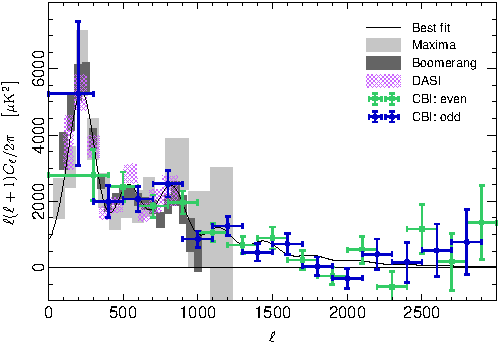
\includegraphics[width=8.8cm]{PlanckFig_lineplot_IDL_88mm.pdf}
\caption{\fcaption} 
\end{figure}

\begin{figure*}
\sidecaption
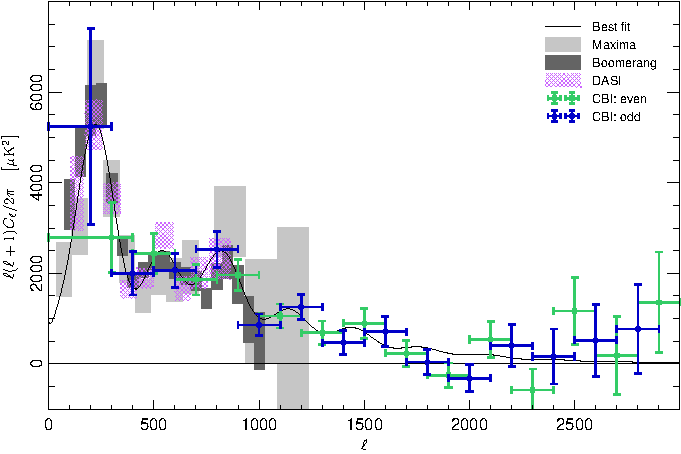
\includegraphics[width=12cm]{PlanckFig_lineplot_IDL_120mm.pdf}
\caption{\fcaption}
\end{figure*}

\begin{figure*}
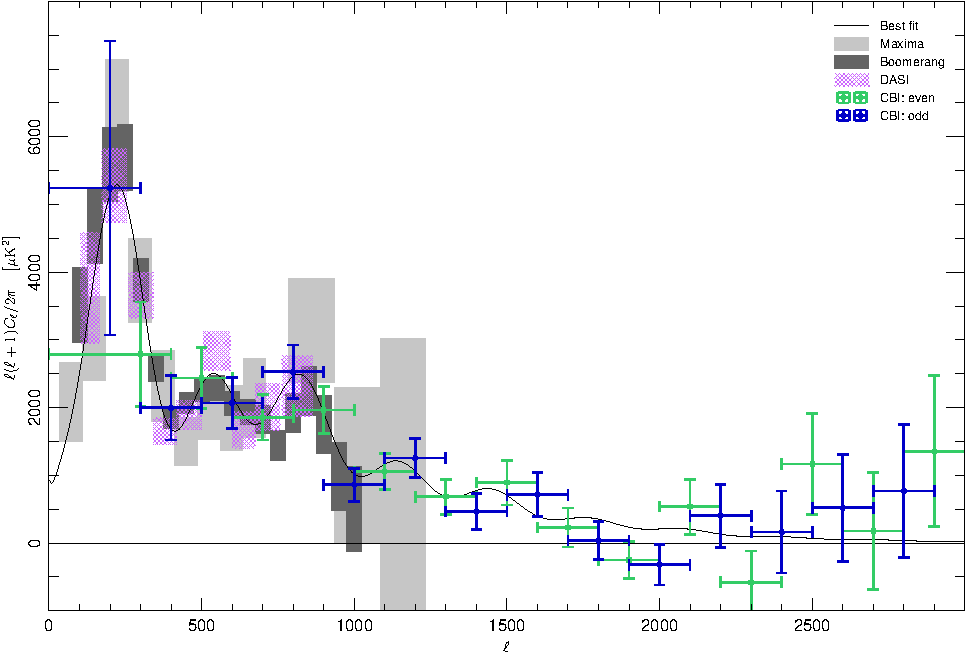
\includegraphics[width=18cm]{PlanckFig_lineplot_IDL_180mm.pdf}
\caption{\fcaption}
\end{figure*}

\clearpage

IDL scripts are also given for two-panel (top, bottom) figures.  Here's what they look like.


\begin{figure}[h]
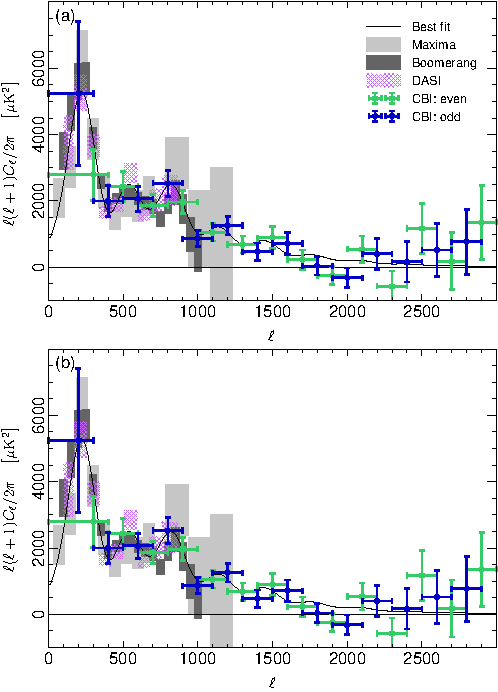
\includegraphics[width=8.8cm]{PlanckFig_lineplot_IDL_2x88mm.pdf}
\caption{\fcaption} 
\end{figure}

\begin{figure*}
\sidecaption
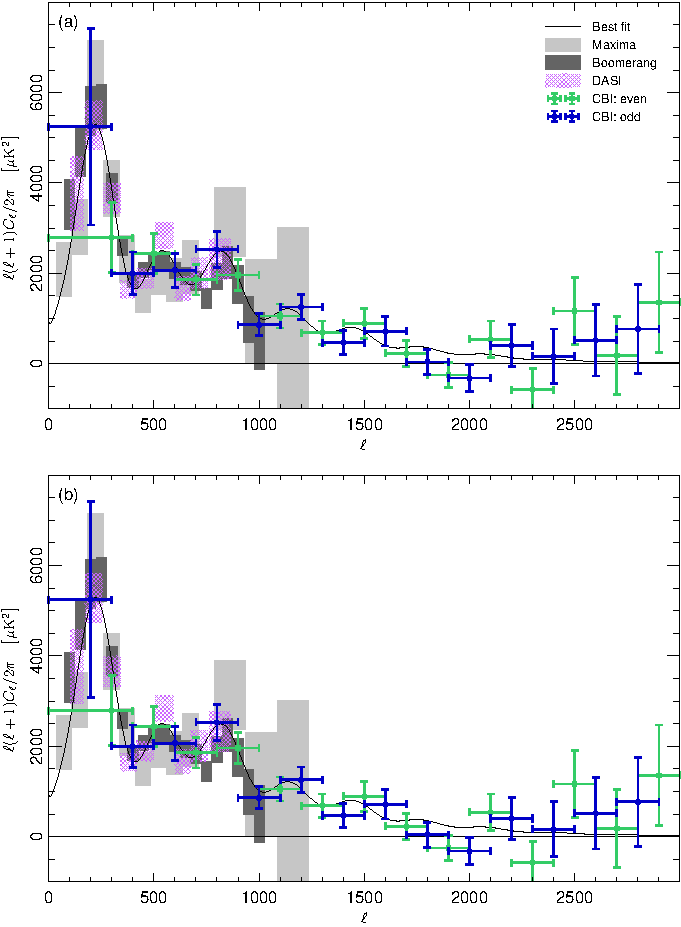
\includegraphics[width=12cm]{PlanckFig_lineplot_IDL_2x120mm.pdf}
\caption{\fcaption}
\end{figure*}

\begin{figure*}
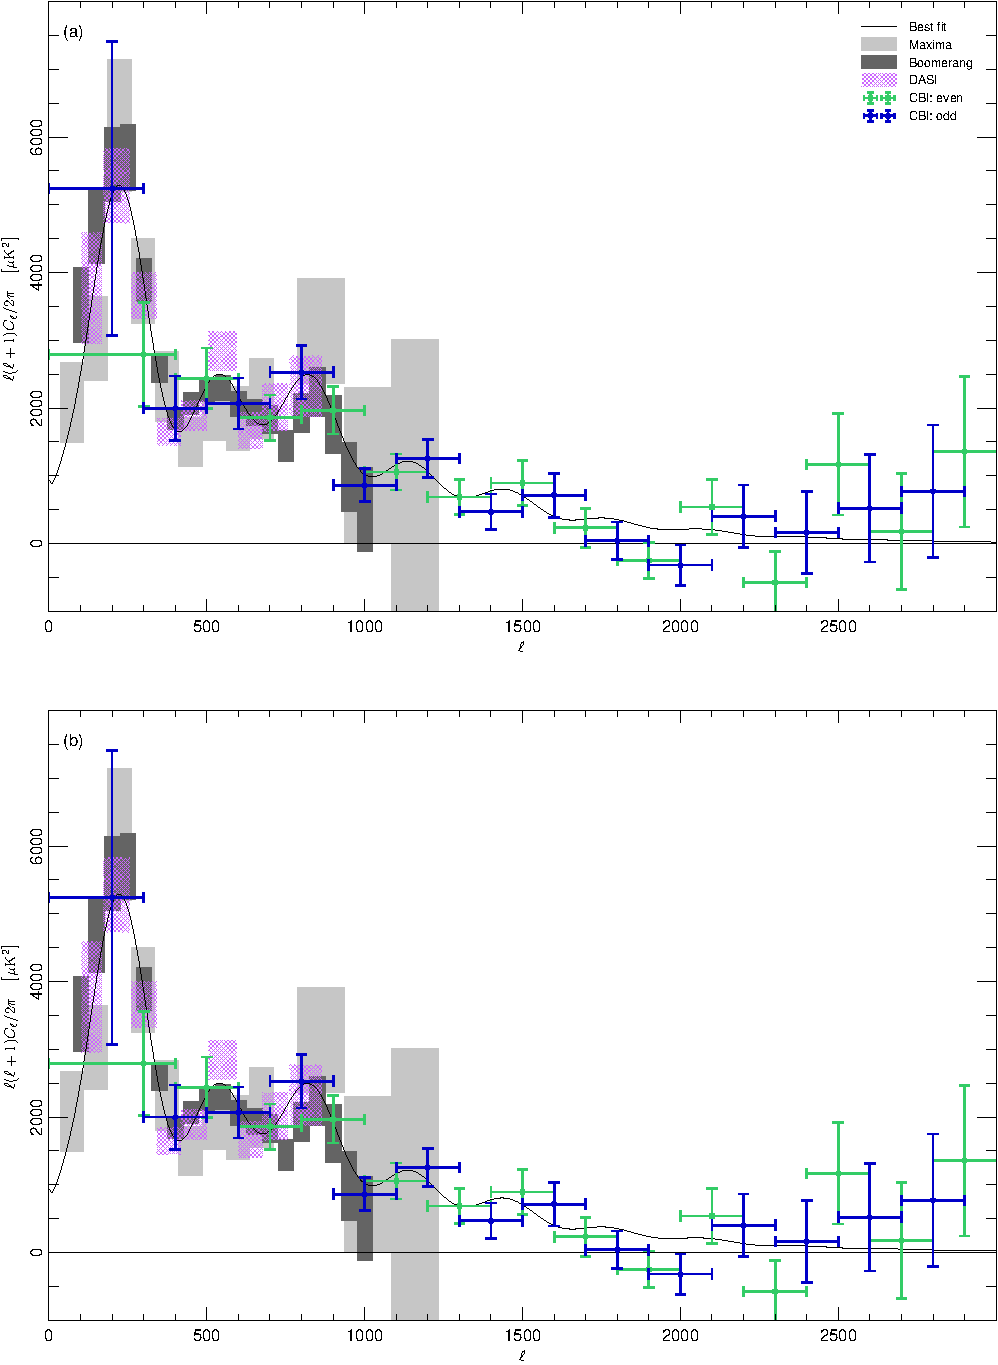
\includegraphics[width=18cm]{PlanckFig_lineplot_IDL_2x180mm.pdf}
\caption{\fcaption}
\end{figure*}

\clearpage





\subsection{Python}

The three equivalent figures as produced by Python are shown in Figs.~7--9.


\begin{figure}[h]
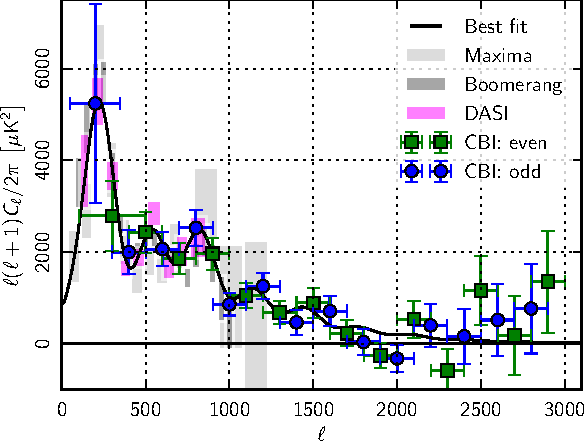
\includegraphics[width=8.8cm]{PlanckFig_lineplot_python_88mm.pdf}
\caption{\fcaption} 
\end{figure}


\begin{figure*}[h]
\sidecaption
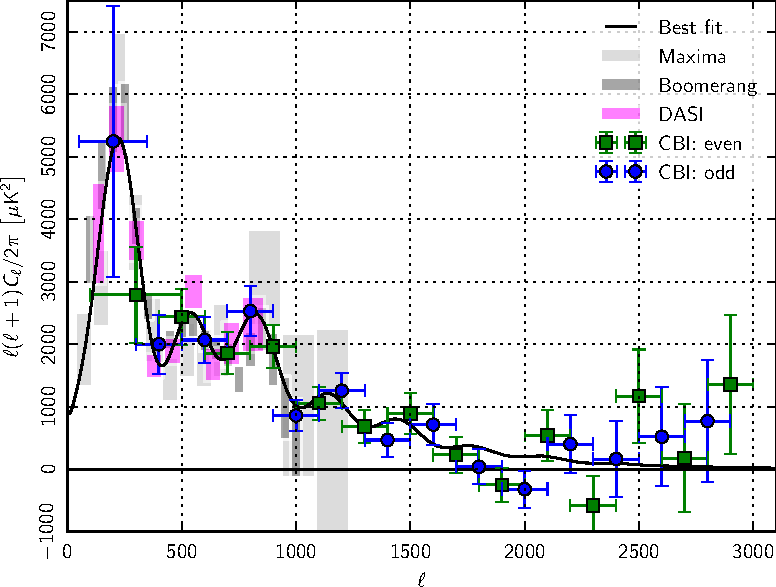
\includegraphics[width=12cm]{PlanckFig_lineplot_python_120mm.pdf}
\caption{\fcaption}
\end{figure*}

\begin{figure*}[t]
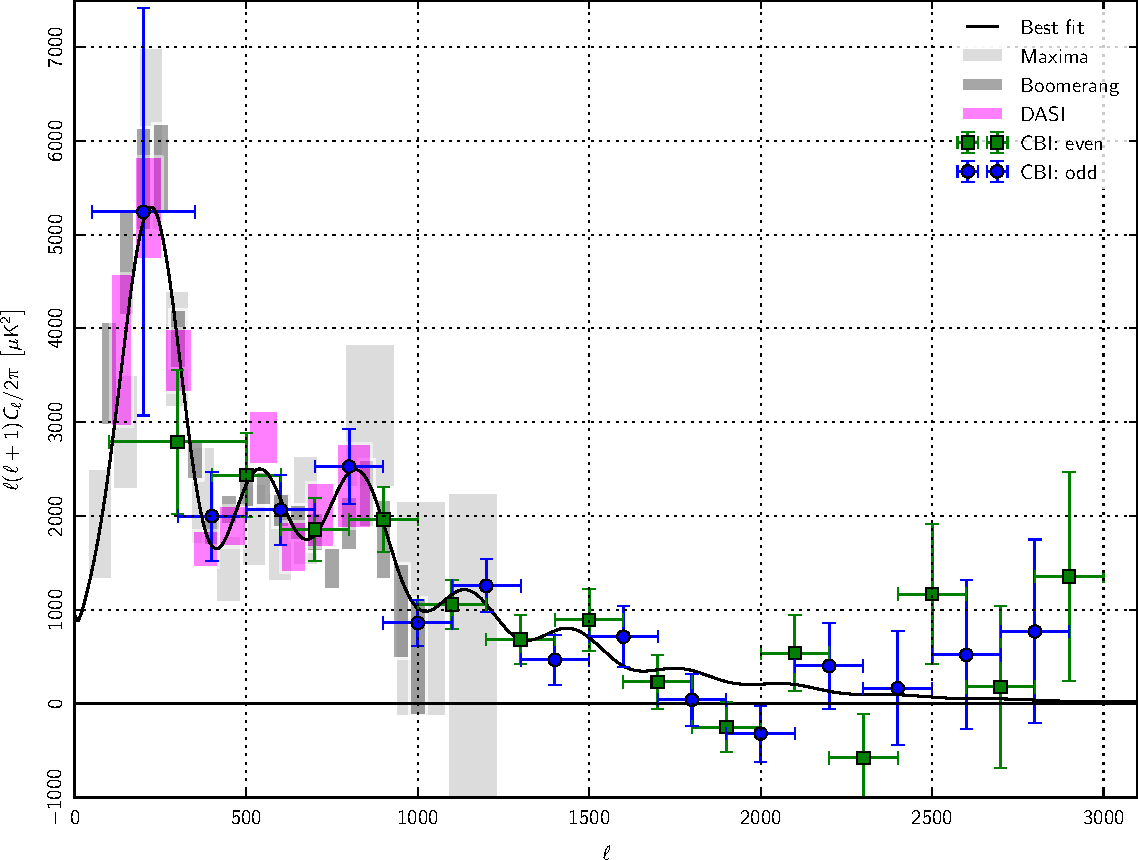
\includegraphics[width=18cm]{PlanckFig_lineplot_python_180mm.pdf}
\caption{\fcaption}
\end{figure*}

\clearpage











\section{Maps}

An example map is shown in the three standard sizes, and also with two different colour tables.


\subsection{Python}


\begin{figure}[h]
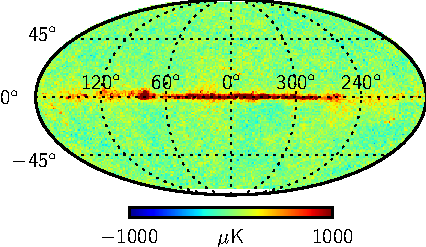
\includegraphics[width=8.8cm]{PlanckFig_map_python_88mm}
\caption{\label{fig:gainCurve} Mollview, 88\,mm wide.  The map itself is bitmapped, but all text is vectorized.} 
\end{figure}

\begin{figure}[h]
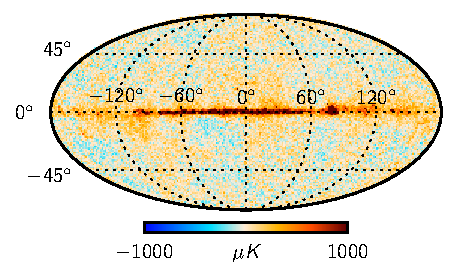
\includegraphics[width=8.8cm]{PlanckFig_map_colombi1_88mm}
\caption{\label{fig:gainCurve} Mollview, 88\,mm wide.  The map itself is bitmapped, but all text is vectorized.} 
\end{figure}



\begin{figure*}[h]
\sidecaption
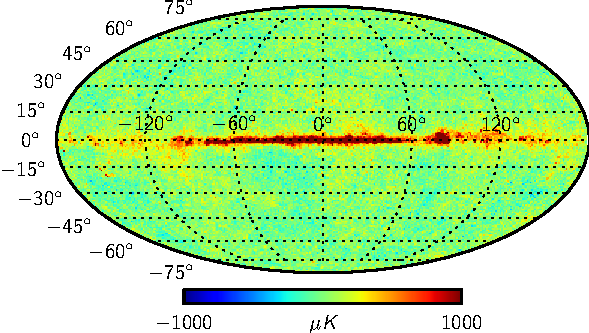
\includegraphics[width=12cm]{PlanckFig_map_python_120mm}
\caption{\label{fig:gainCurve} Mollview, 120\,mm wide.  The map itself is bitmapped, but all text is vectorized.} 
\end{figure*}

\begin{figure*}[h]
\sidecaption
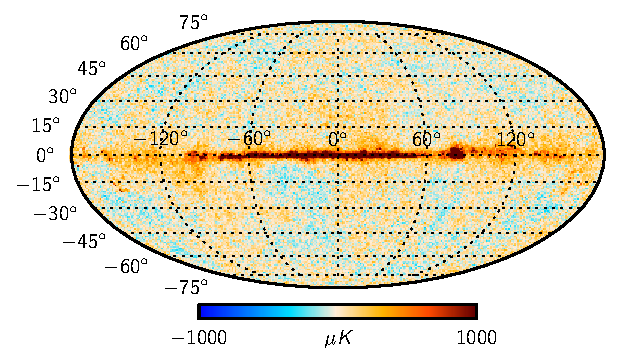
\includegraphics[width=12cm]{PlanckFig_map_colombi1_120mm}
\caption{\label{fig:gainCurve} Mollview, 120\,mm wide.  The map itself is bitmapped, but all text is vectorized.} 
\end{figure*}



\begin{figure*}[H!b]
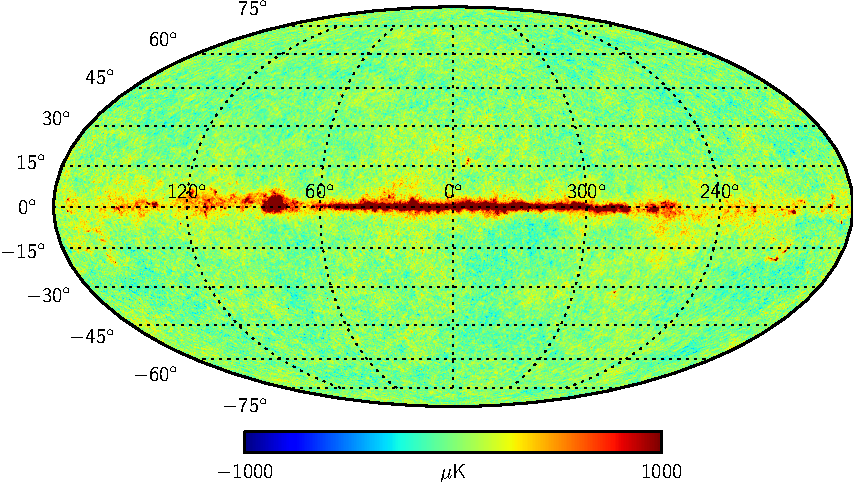
\includegraphics[width=18cm]{PlanckFig_map_python_180mm}
\caption{\label{fig:gainCurve} Mollview, 180\,mm wide.  The map itself is bitmapped, but all text is vectorized.}
\end{figure*}

\begin{figure*}[H!b]
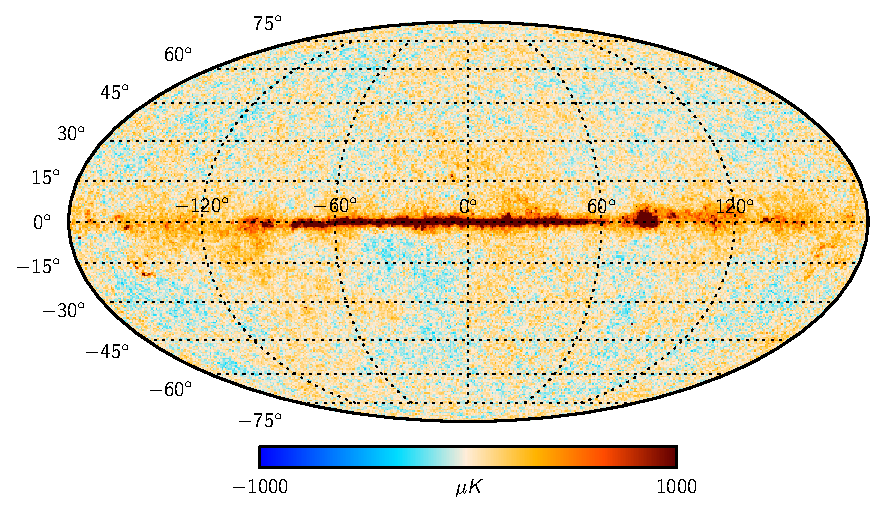
\includegraphics[width=18cm]{PlanckFig_map_colombi1_180mm}
\caption{\label{fig:gainCurve} Mollview, 180\,mm wide.  The map itself is bitmapped, but all text is vectorized.}
\end{figure*}


\clearpage








\section{Parameter-type plots}


\begin{figure}[h]
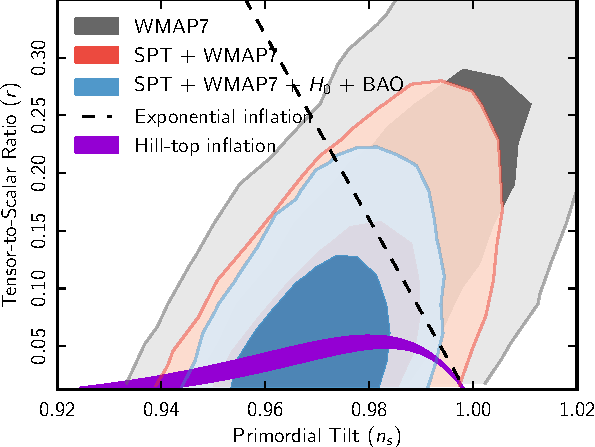
\includegraphics[width=\columnwidth]{PlanckFig_parameters_python_88mm}
\caption{\label{fig:gainCurve}Parameters, 88\,mm wide.  The use of transparency is essential for clarity.}
\end{figure}

\begin{figure*}[H!b]
\sidecaption
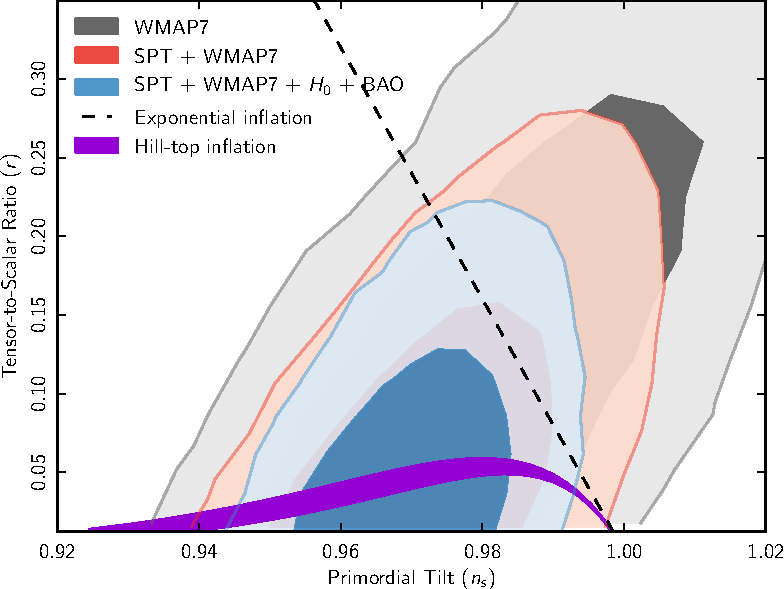
\includegraphics[width=12cm]{PlanckFig_parameters_python_120mm}
\caption{\label{fig:gainCurve}Parameters, 120\,mm wide.  The use of transparency is essential for clarity.}
\end{figure*}

\begin{figure*}[H!b]
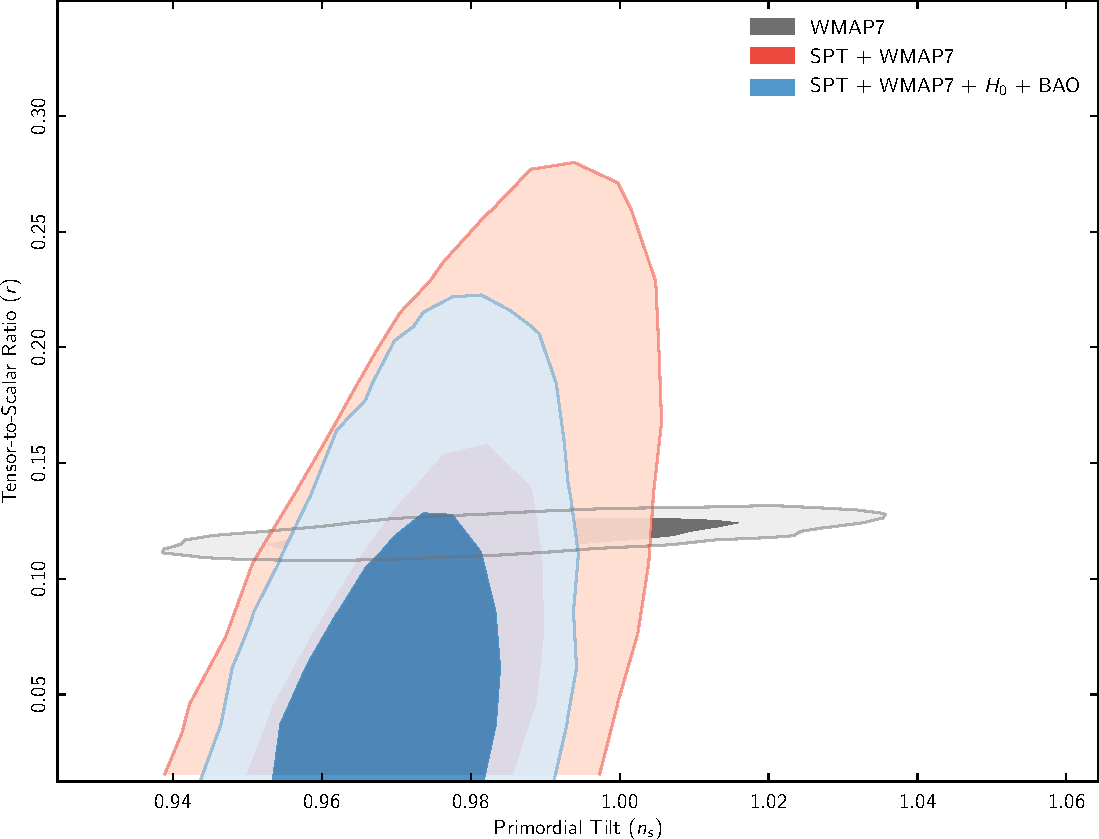
\includegraphics[width=18cm]{PlanckFig_parameters_python_180mm}
\caption{\label{fig:gainCurve}Parameters, 180\,mm wide.  The use of transparency is essential for clarity.}
\end{figure*}

\end{document}
